\section{Competidores} % 3.4 Top performers
\urgent[inline]{List other top-selling games in the same market. Provide sales
figures, release dates, information on sequels and platforms, as well as brief
descriptions of each title.}

\subsection{Ultimate Chicken Horse}

\href{https://www.cleverendeavourgames.com/ultimate-chicken-horse/}{\emph{Ultimate
Chicken Horse}}, desarrollado y publicado por \emph{Clever Endeavour Games} en
el 2016, es un videojuego festivo de plataformas en el que el jugador debe
hacerse de trampas y obstáculos para colocarlas en el nivel y así evitar que los
compañeros de juego consigan llegar a la meta. Sin embargo, el propio jugador no
es inmune a sus trampas y, por tanto, debe evitar caer también en ellas.

El juego está disponible para PC, Nintendo Switch, XBOX One y PS4 y su modelo de
negocio es Buy-to-Play con DLCs. Se estima que ha realizado unas ganancias de
$6.1$ millones de dólares \footnote{Según aparece en
\url{https://games-stats.com/steam/game/ultimate-chicken-horse/}}

% \textbf{Capturas:}
\begin{figure}[H]
    \centering
    \begin{minipage}{0.40\textwidth}
        \centering
        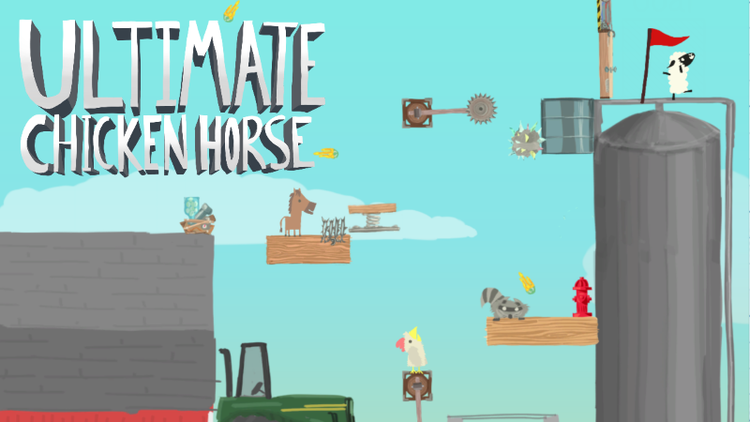
\includegraphics[width=1.0\textwidth]{5-Cuerpo/Chapter3/UCH1.png} %
        \subcaption{Pantalla principal del juego}
        \label{UCH-Inicio}
    \end{minipage}\hfill
    \begin{minipage}{0.40\textwidth}
        \centering
        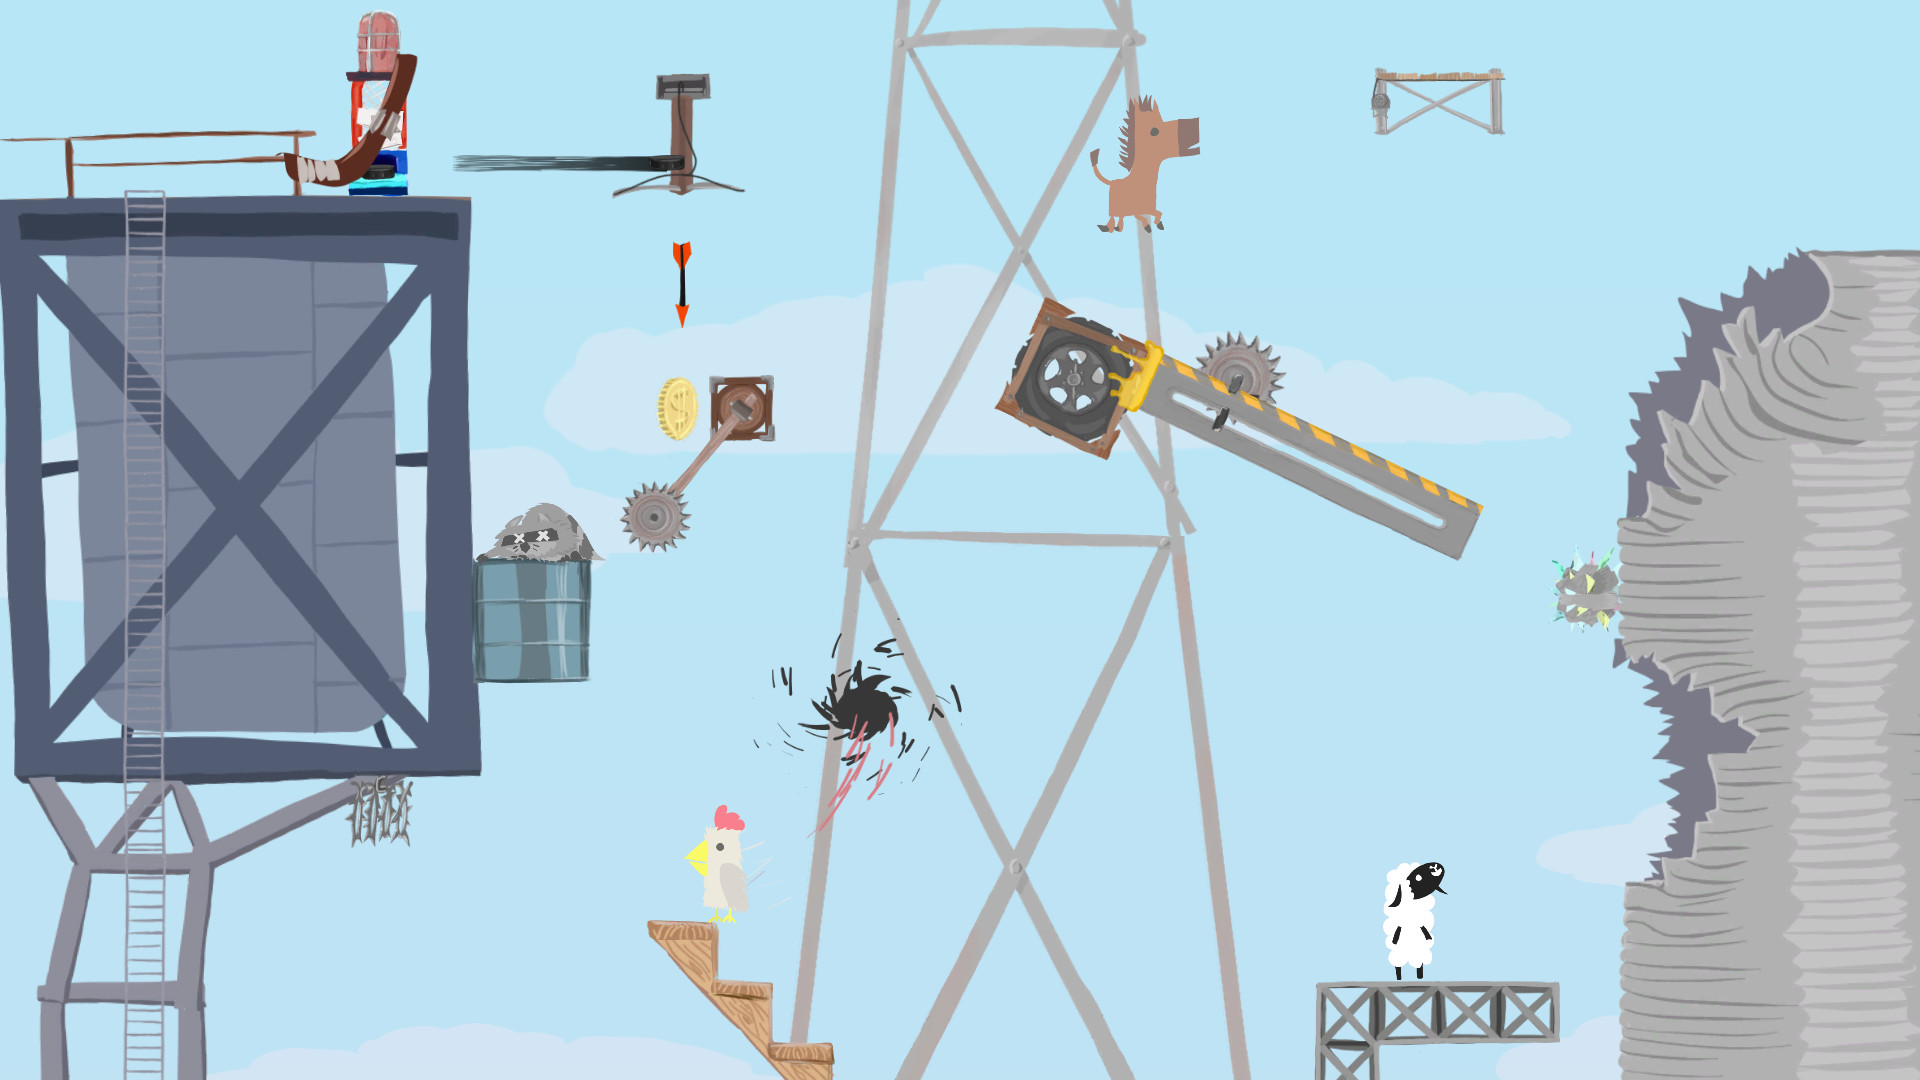
\includegraphics[width=1.0\textwidth]{5-Cuerpo/Chapter3/UCH2.jpg} %
        \subcaption{Algunos jugadores (animales) y obstáculos}
        \label{UCH-Jugadores}
    \end{minipage}
    \centering
    \begin{minipage}{0.40\textwidth}
        \centering
        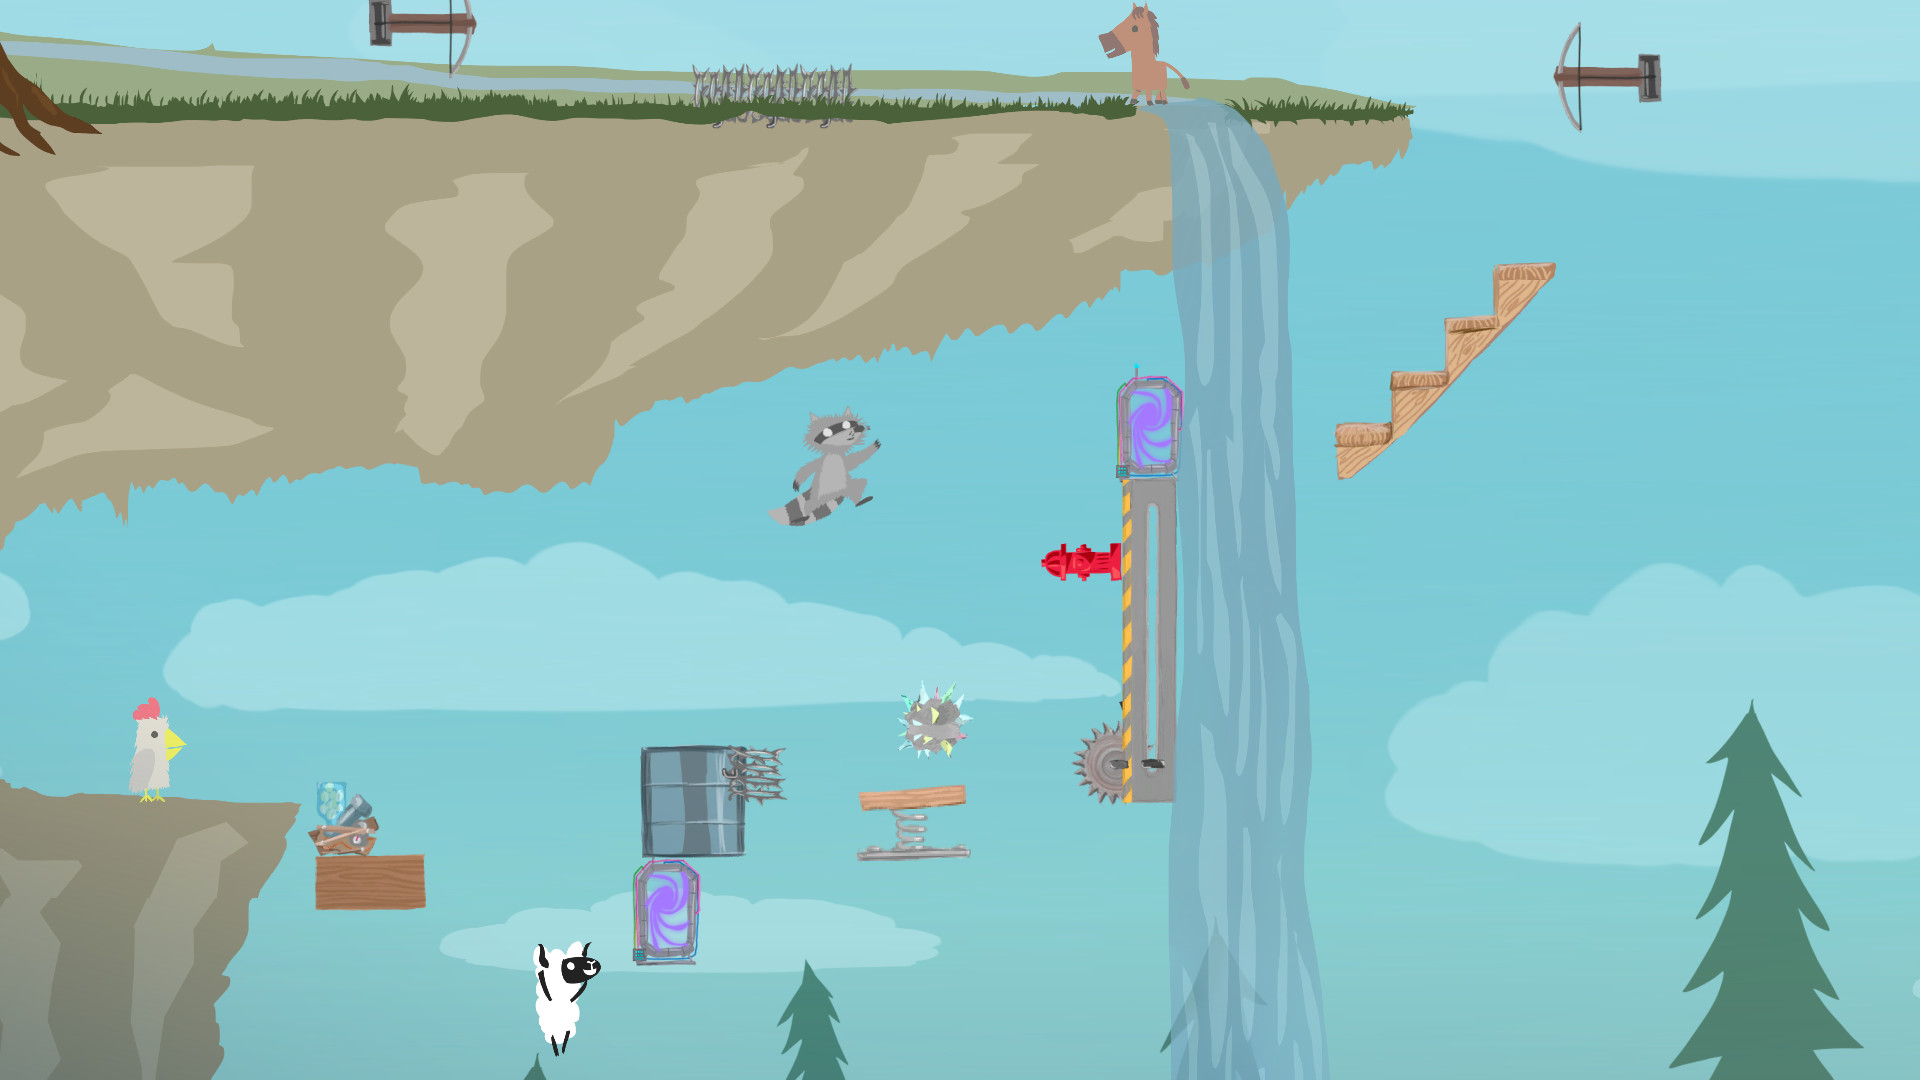
\includegraphics[width=1.0\textwidth]{5-Cuerpo/Chapter3/UCH3.jpg} %
        \subcaption{Un jugador cayendo hacia al vacío y otro saltando}
        \label{UCH-Muerte}
    \end{minipage}
    \caption{Capturas de Ultimate Chicken Horse}
\end{figure}

\subsection{Jackbox Party Packs}

\href{https://www.jackboxgames.com/}{\emph{Jackbox Party Packs}}, desarrollados
y publicados por \emph{Jackbox Games, Inc.} desde el 2014, son una serie de
videojuegos cada uno compuesto por una serie de minijuegos distintos que se
pueden jugar online sin necesidad de que todos los participantes hayan comprado
el juego.

El juego está disponible para PC, Nintendo Switch, XBOX One, PS4, iOS y Stadia.
Su modelo de negocio es Buy-to-Play. Se estima que la séptima instancia del
juego ha llegado a generar unas ganancias de aproximadamente $1.5$ millones de
dólares \footnote{Según aparece en
\url{https://games-stats.com/steam/game/the-jackbox-party-pack-7}}

% \textbf{Capturas:}
\begin{figure}[H]
    \centering
    \begin{minipage}{0.40\textwidth}
        \centering
        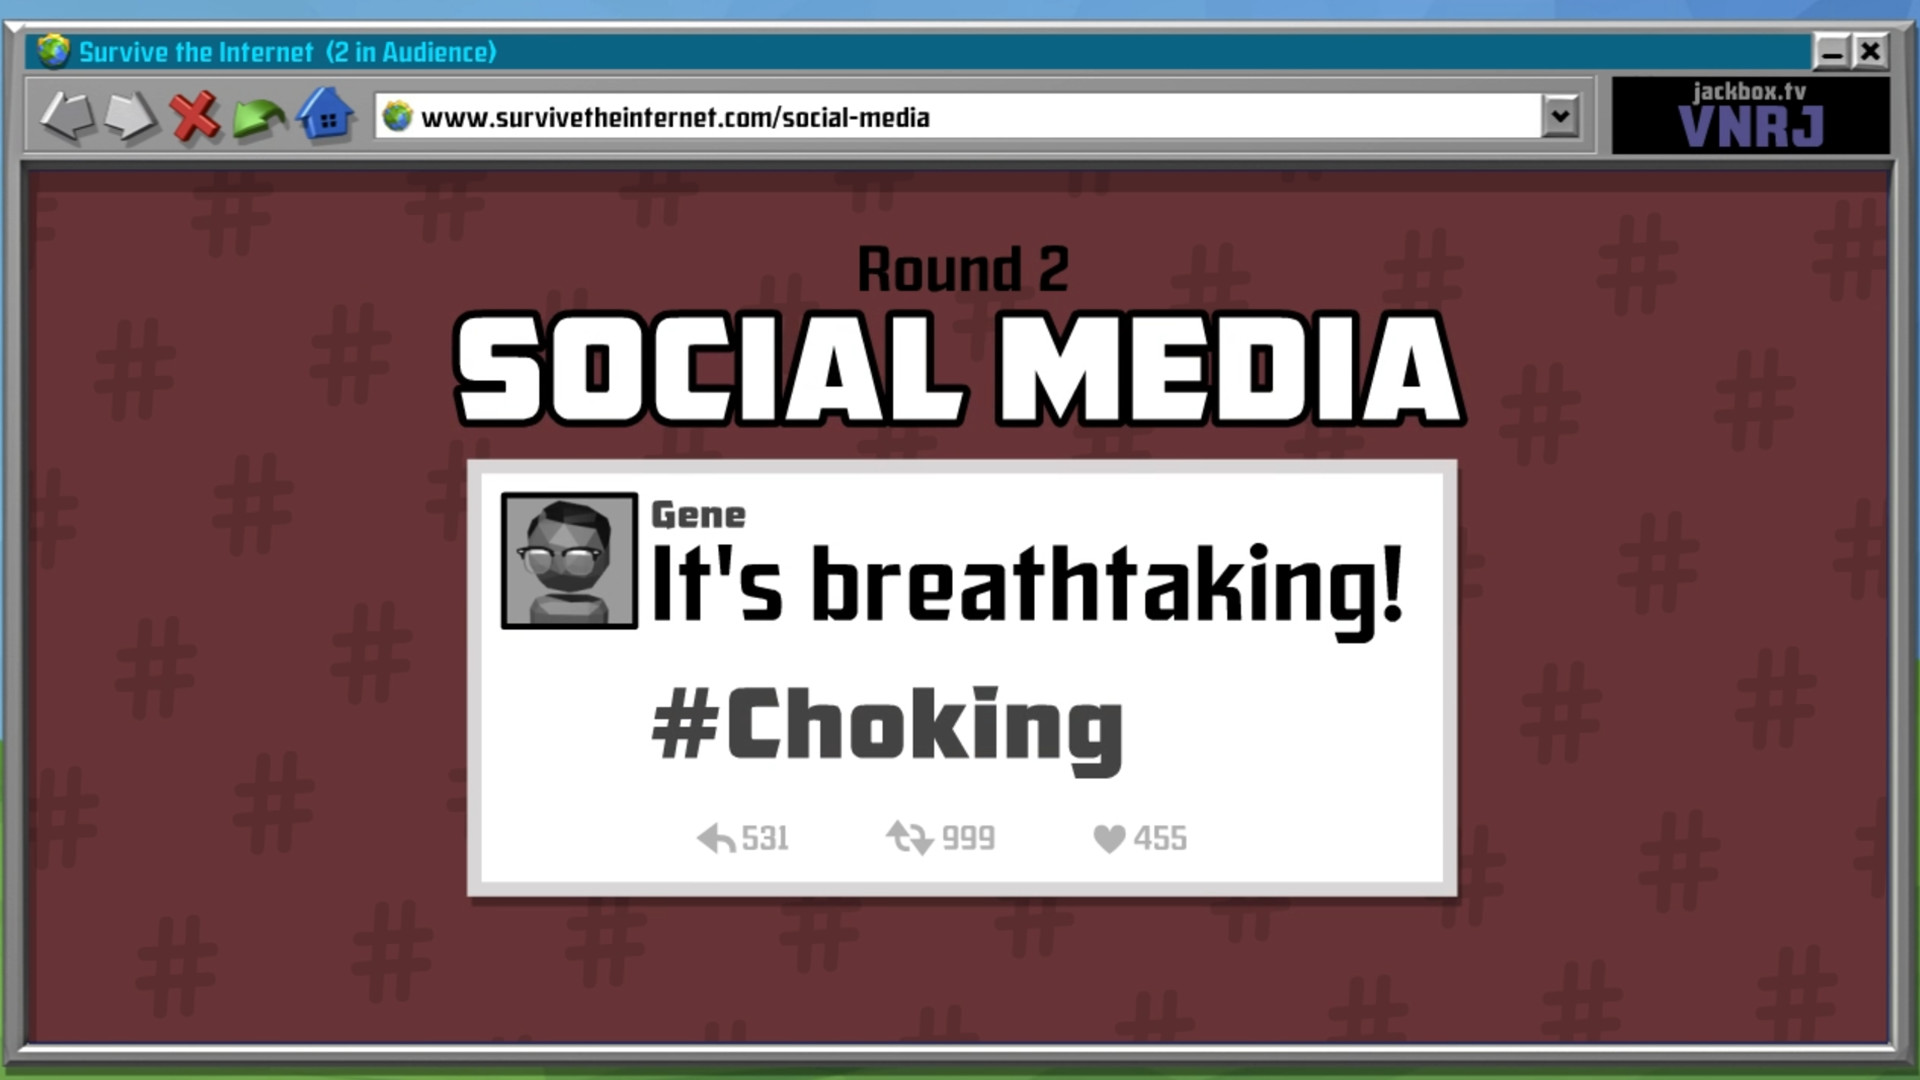
\includegraphics[width=1.0\textwidth]{5-Cuerpo/Chapter3/JPP1.jpg} %
        \subcaption{Un minijuego de uno de los packs}
        \label{JPP-Internet}
    \end{minipage}\hfill
    \begin{minipage}{0.40\textwidth}
        \centering
        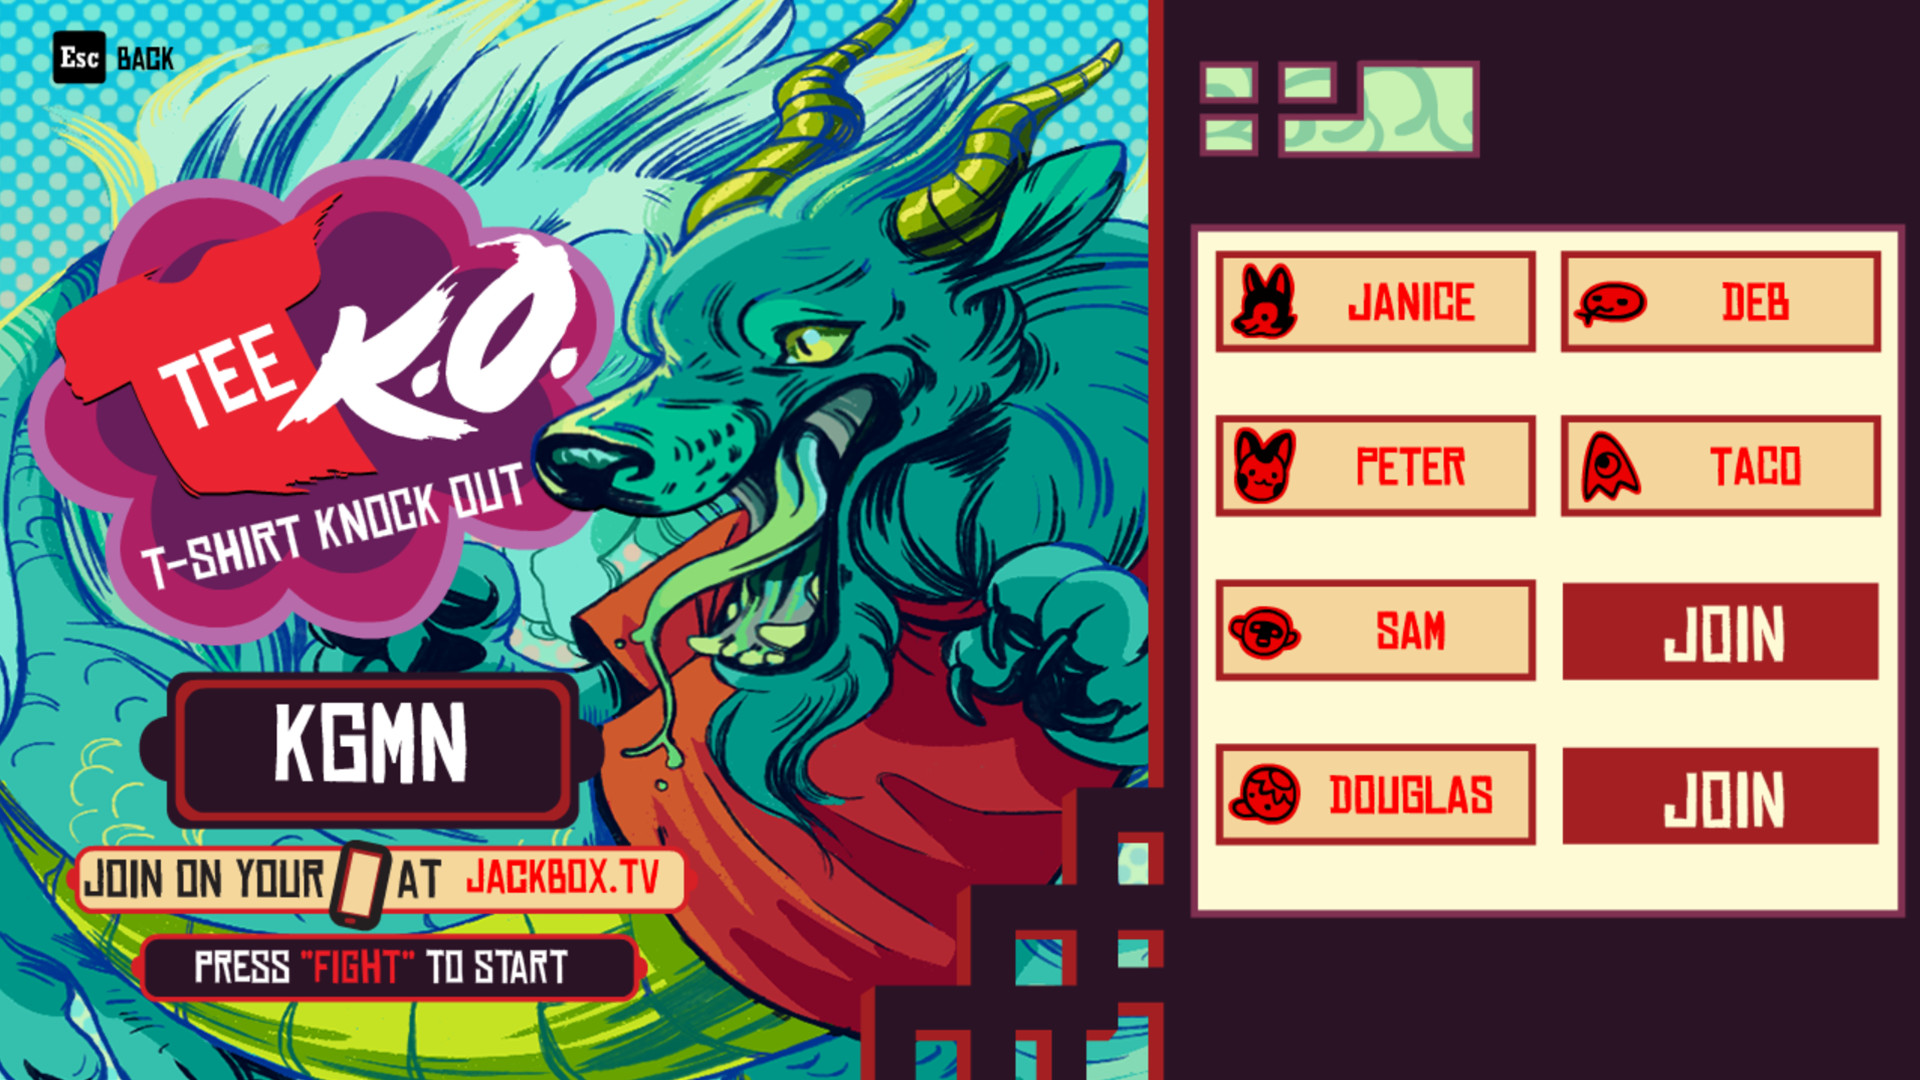
\includegraphics[width=1.0\textwidth]{5-Cuerpo/Chapter3/JPP2.jpg} %
        \subcaption{Pantalla de inicio de otro minijuego}
        \label{JPP-Inicio}
    \end{minipage}
    \centering
    \begin{minipage}{0.40\textwidth}
        \centering
        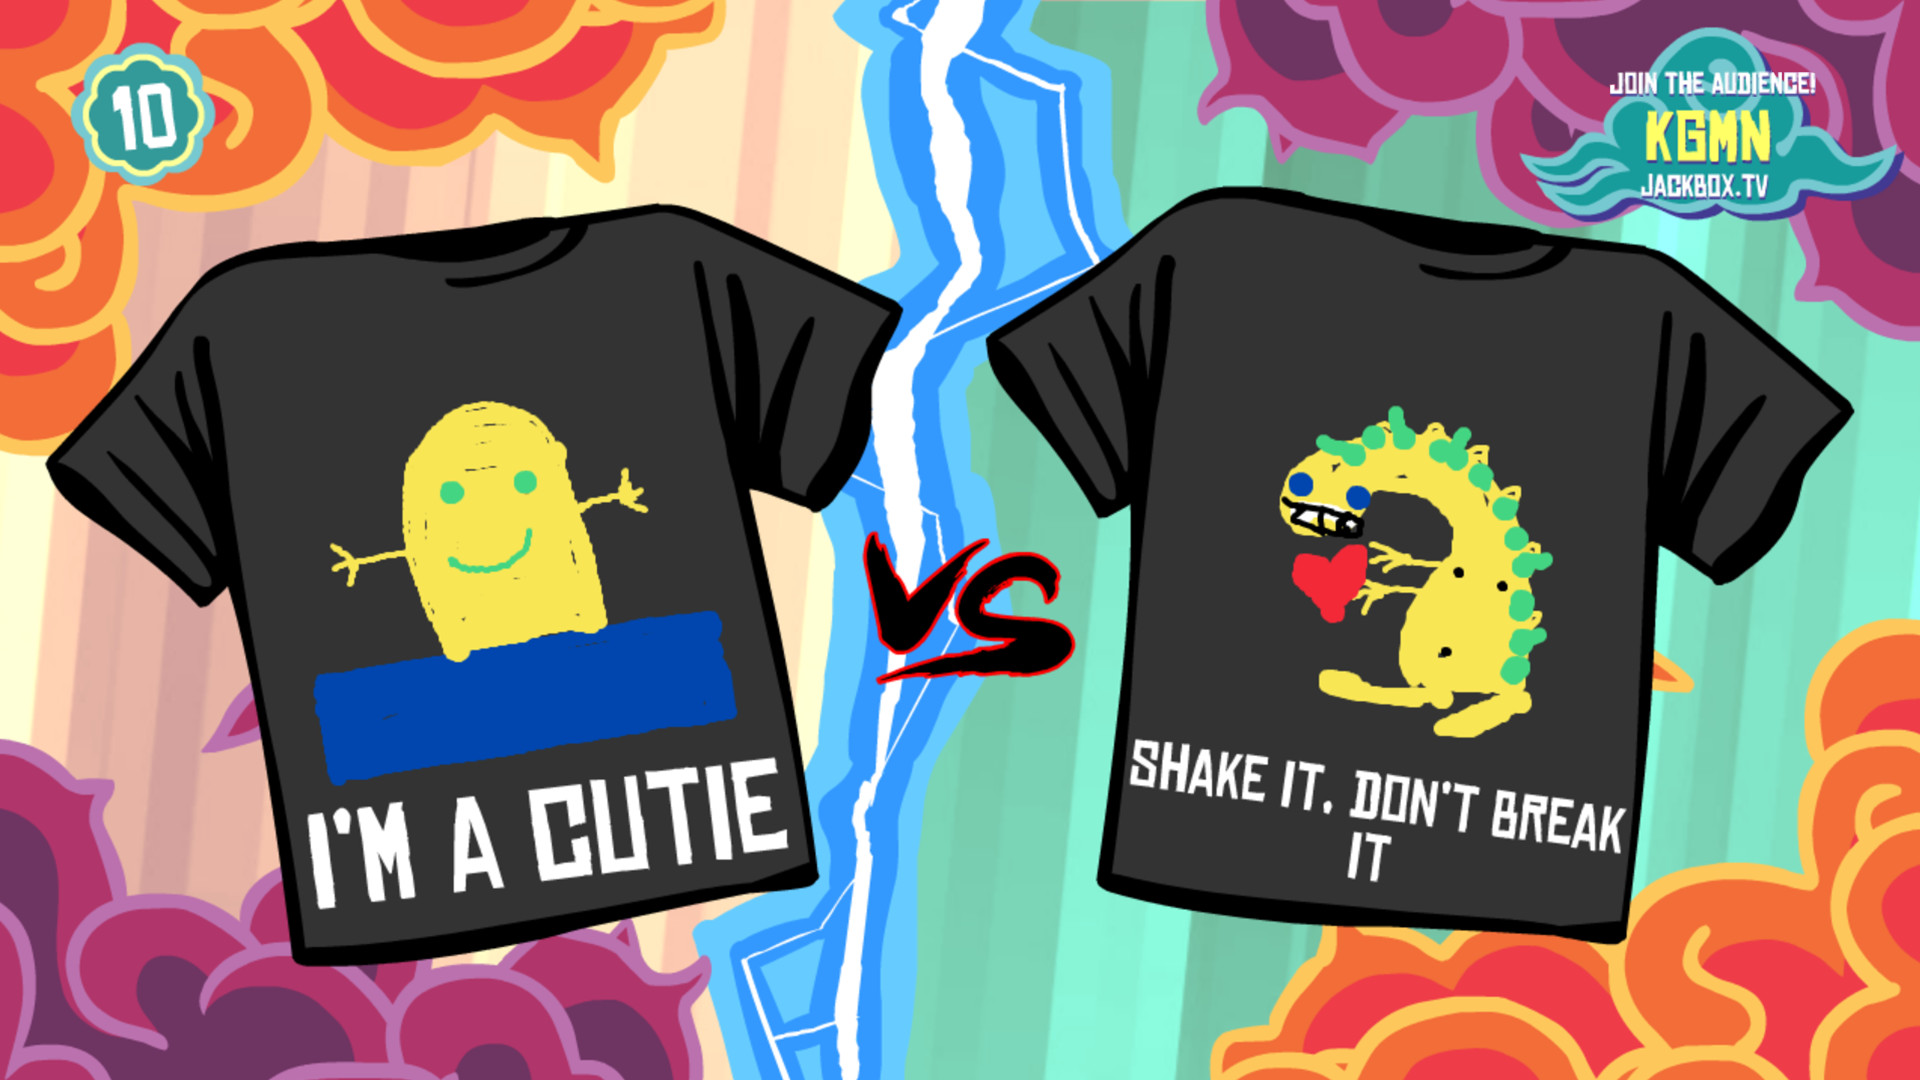
\includegraphics[width=1.0\textwidth]{5-Cuerpo/Chapter3/JPP3.jpg} %
        \subcaption{Otro minijuego de uno de los packs}
        \label{JPP-Tees}
    \end{minipage}
    \caption{Capturas de varios juegos de los Jackbox Party Packs}
\end{figure}

\subsection{Pummel Party}

\href{http://www.rebuiltgames.com/}{\emph{Pummel Party}}, desarrollado y
publicado por \emph{Rebuilt Games} en el 2018, es un juego festivo multijugador
usando en la que se destruye a tus compañeros con una variedad de objetos y se
compite por puntos en una colección de minijuegos distintos.


Este videojuego está disponible sólo para PC, y más especificamente para
sistemas Windows. Se estima que ha generado una ganancia de aproximadamente
$8.2$ millones de dólares. \footnote{Según aparece en
\url{https://games-stats.com/steam/game/pummel-party/}}

% \textbf{Capturas:}
\begin{figure}[H]
    \centering
    \begin{minipage}{0.40\textwidth}
        \centering
        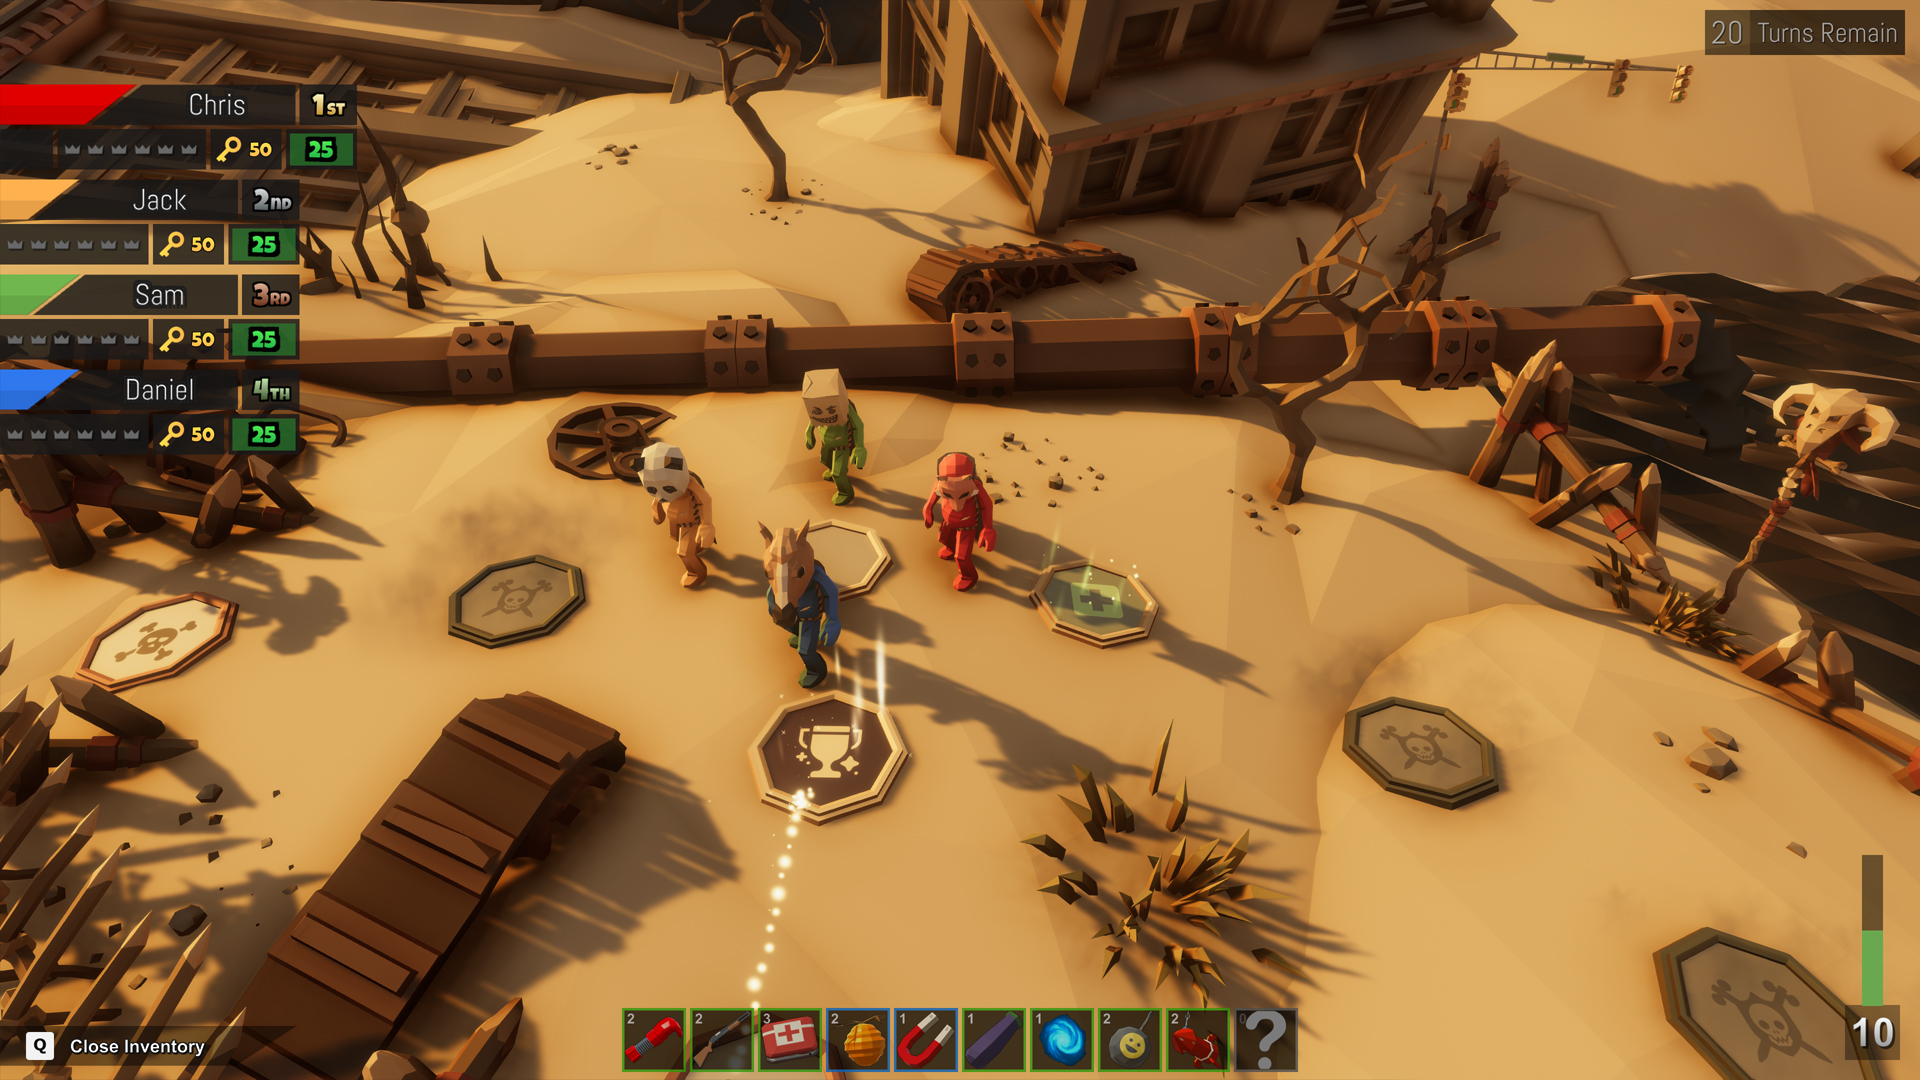
\includegraphics[width=1.0\textwidth]{5-Cuerpo/Chapter3/PMP1.jpg} %
        \subcaption{El modo tablero de Pummel Party}
        \label{PMP-Tablero}
    \end{minipage}\hfill
    \begin{minipage}{0.40\textwidth}
        \centering
        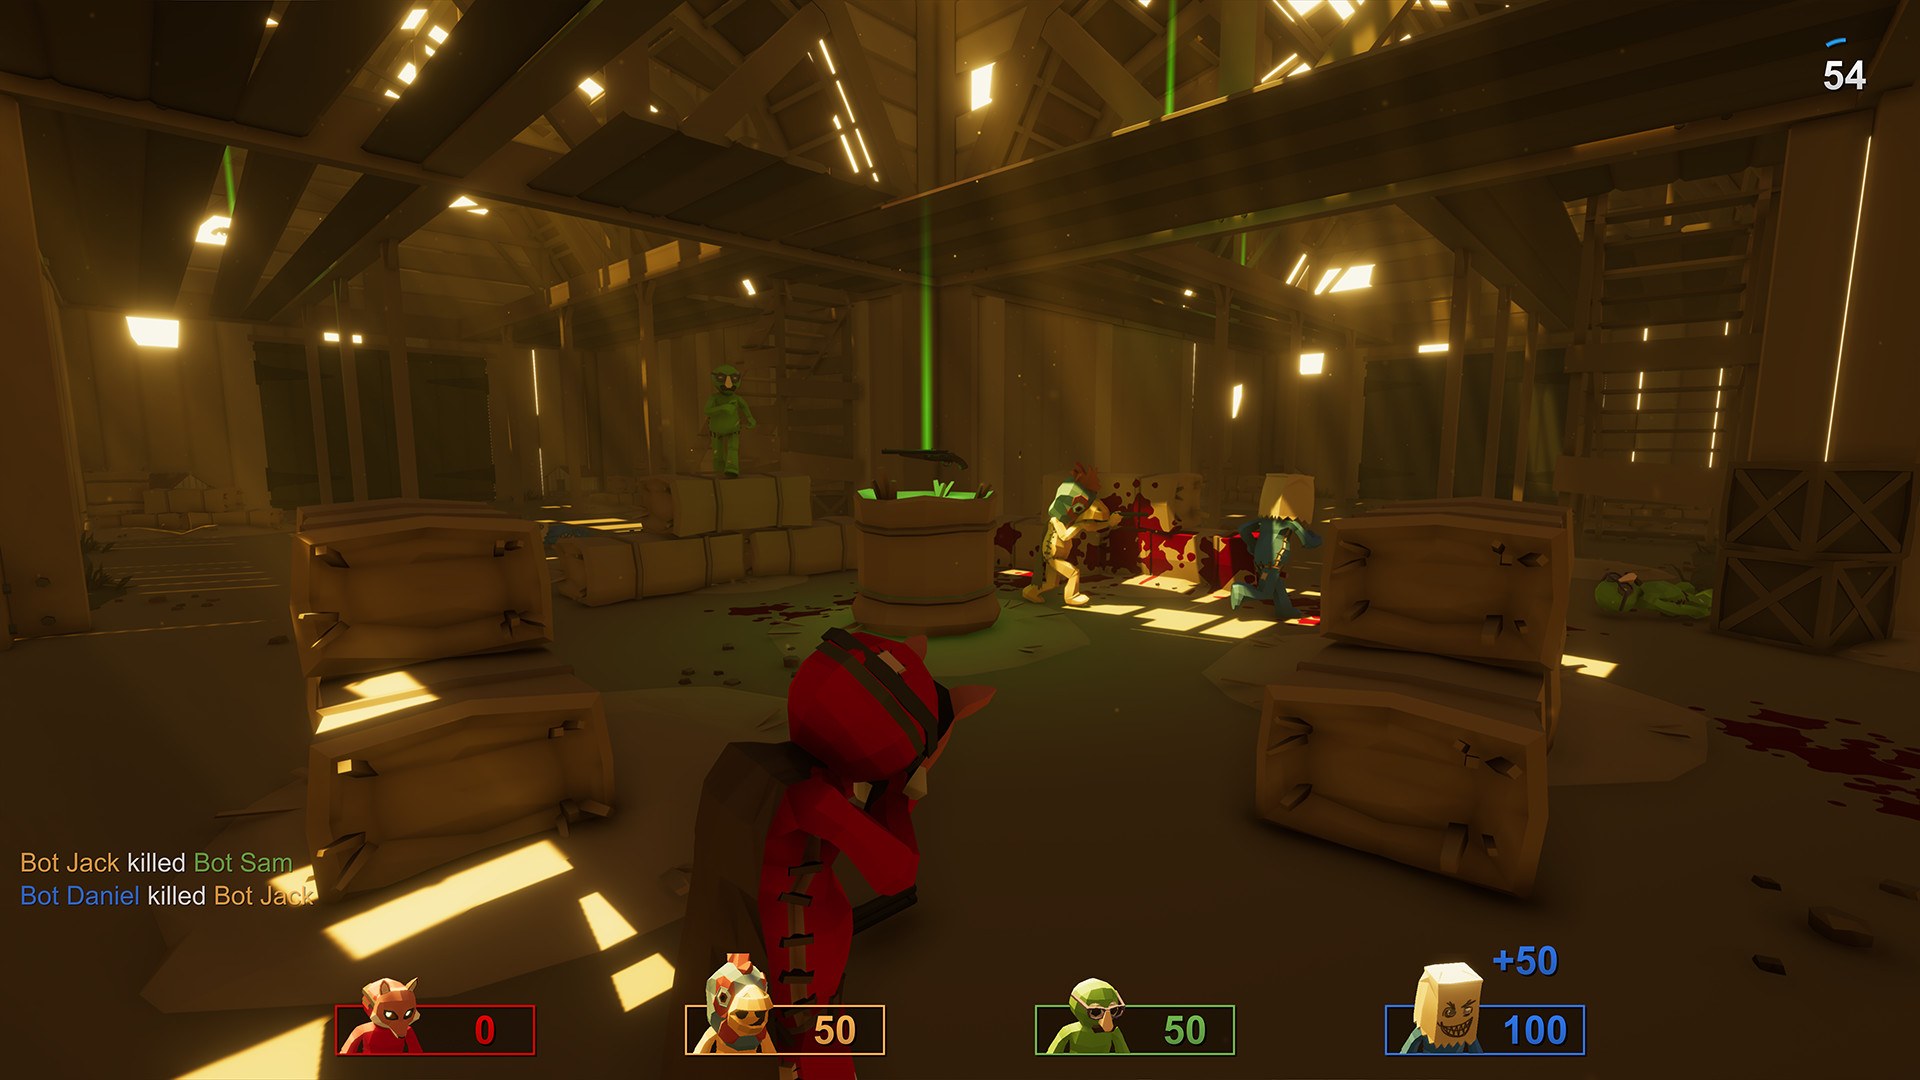
\includegraphics[width=1.0\textwidth]{5-Cuerpo/Chapter3/PMP2.jpg} %
        \subcaption{Un minijuego de tipo shooter}
        \label{PMP-Shooter}
    \end{minipage}
    \centering
    \begin{minipage}{0.40\textwidth}
        \centering
        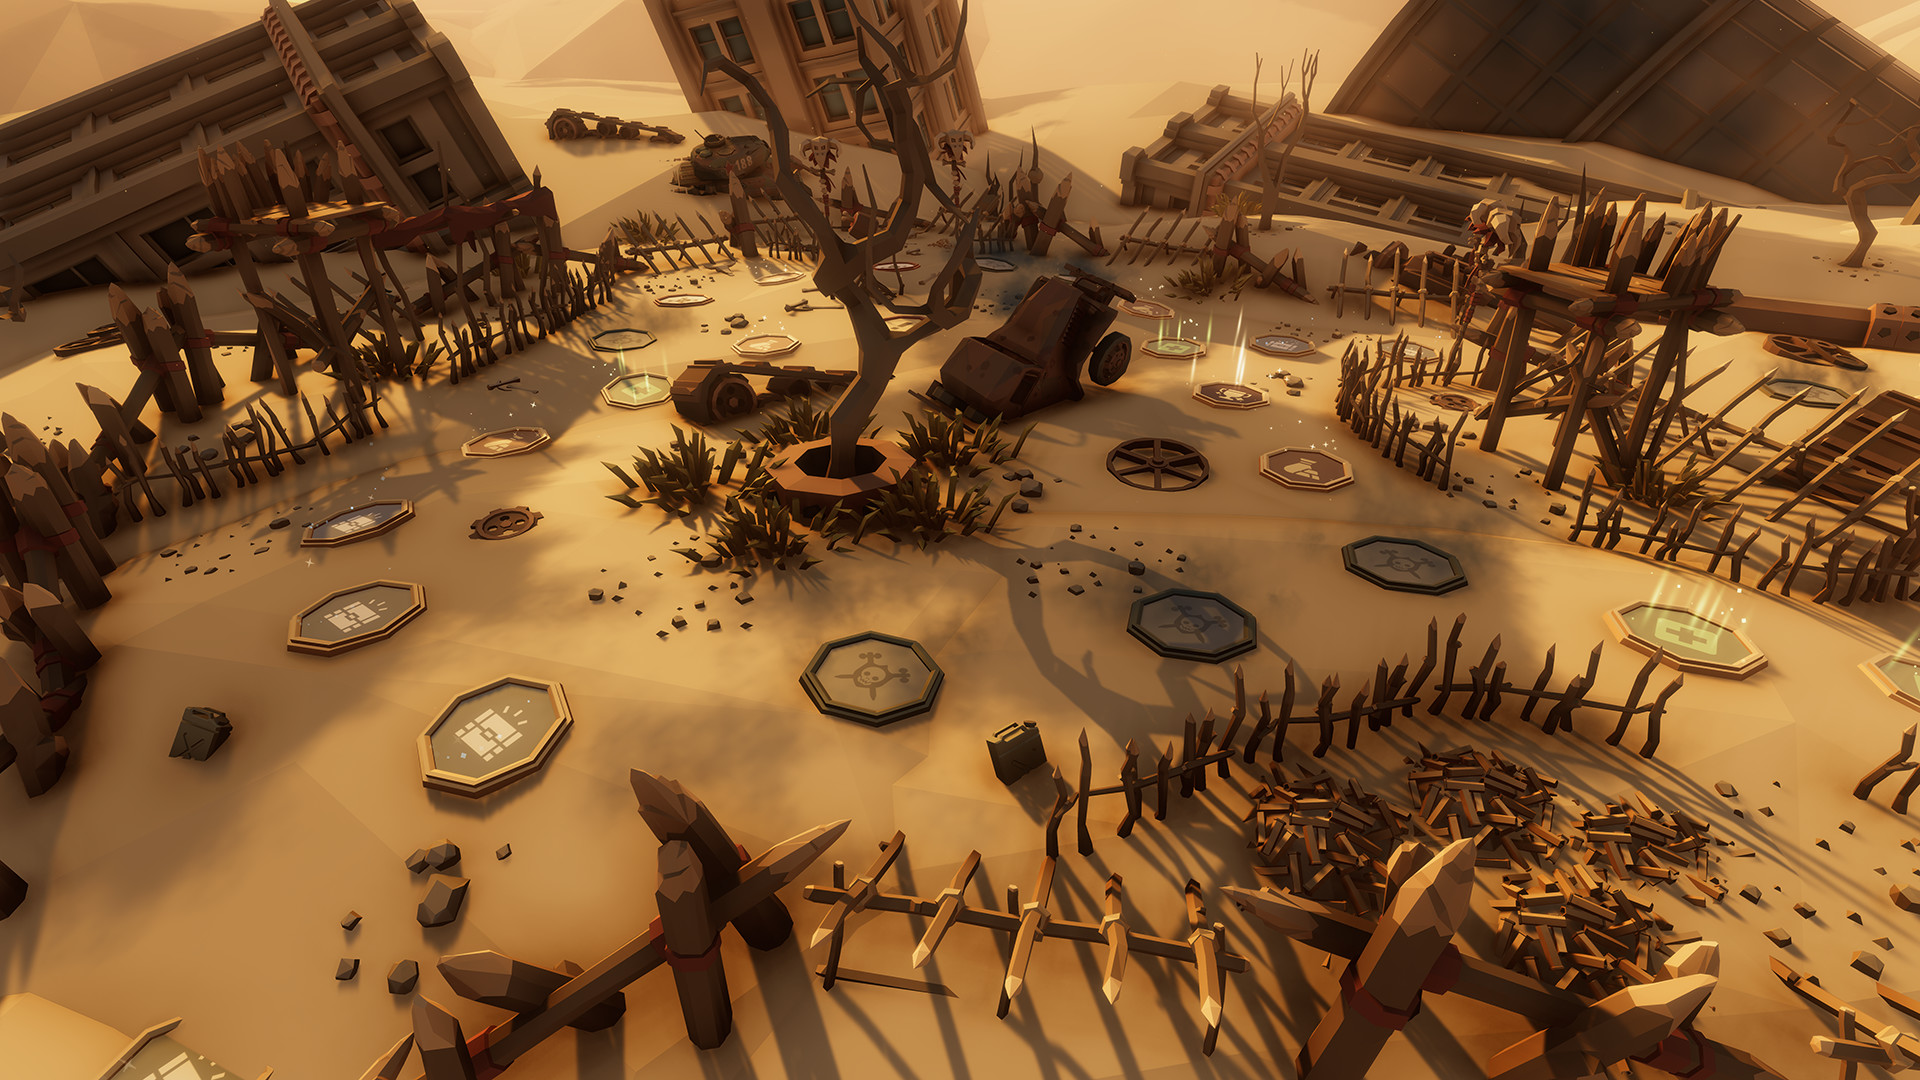
\includegraphics[width=1.0\textwidth]{5-Cuerpo/Chapter3/PMP3.jpg} %
        \subcaption{Uno de los paisajes de un tablero}
        \label{PMP-Paisaje}
    \end{minipage}
    \caption{Capturas de Pummel Party}
\end{figure}